%=== CHAPTER FOUR ===
%% The estimator and controller models, the two optimal control problems, the
%% continuous payload interface, inner-loop scheduling and the grasp/release
%% lifecycle.  Rewritten 2026-10-30 against the 14-state mass-only
%% implementation; restructured 2026-11-05: the estimator and controller models
%% (formerly split between Chapter 3 and this chapter) are collected in
%% Section 4.2, the reduced velocity--mass estimator is the deployed default, and
%% the two optimal control problems are adjacent.  Labels are unchanged.

\chapter{The MHE--NMPC Framework}
\label{ch:framework}
\begin{spacing}{1.5}
\setlength{\parskip}{0.22in}

Chapter~\ref{ch:model} established \emph{what} is estimated and why. This
chapter states \emph{how}. Section~\ref{sec:frame:models} collects the models in
one place --- the deployed velocity--mass estimator, the full-state estimator with
which the evaluation campaigns were flown, and the controller's prediction model.
Sections~\ref{sec:frame:mhe} and \ref{sec:frame:nmpc} give the two optimal
control problems built on them, Section~\ref{sec:frame:interface} the interface
that carries the estimate from one to the other, Section~\ref{sec:frame:omegascale}
the inner-loop scheduling that consumes the same estimate, and
Section~\ref{sec:frame:lifecycle} the logic that decides when the controller may
believe that its payload has gone.

The estimator receives no attach or release notification. The controller's
model parameters follow the estimate continuously, and a release is
\emph{accepted} --- declared complete, with auxiliary states reset --- only on
persistent estimator evidence. Section~\ref{sec:frame:why-eventless} separates
what that acceptance does from what the continuous adaptation does, and
Section~\ref{sec:frame:limits-lifecycle} states what a mass-only lifecycle cannot
do.

\section{Closed-Loop Architecture}\label{sec:frame:arch}

Figure~\ref{fig:architecture} shows the information flow. Three layers are
involved: the physics and flight stack (Gazebo, PX4 software-in-the-loop, and a
magnetic detachable-joint gripper that produces genuine mass and inertia
changes); the inner rate-control loop on the autopilot; and a ROS outer loop
containing the estimator and the predictive controller.

\begin{figure}[ht]
\centering
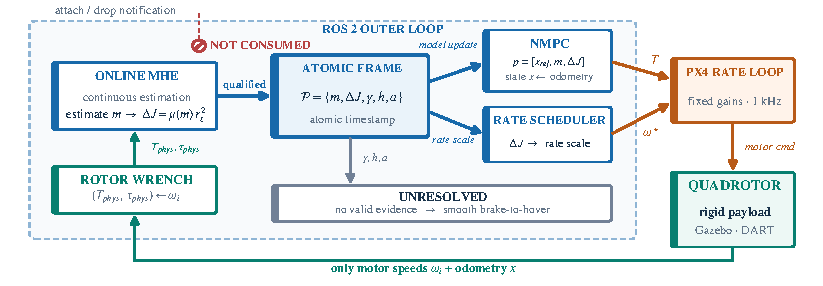
\includegraphics[width=0.98\textwidth]{Figures/fig1_architecture_massonly.pdf}
\caption{System architecture and information flow. The complete pipeline consumes
only rotor speeds and odometry. One atomic, health-gated frame carrying the
composite mass and the inertia increment derived from it drives both the NMPC
model and the continuous body-rate command scheduling. No attach or release
notification enters this path.}
\label{fig:architecture}
\end{figure}

Two properties of this diagram carry the argument of the dissertation.

First, \textbf{the only inputs are odometry and rotor speeds.} The estimator does
not read the controller's intended thrust or torque
(Section~\ref{sec:model:phys}), does not read the gripper's attach or release
record, and does not read the simulator's joint state. The payload truth
available in simulation is used exclusively for offline scoring.

Second, \textbf{there is exactly one interface.} The estimator publishes a single
atomic frame (Section~\ref{sec:frame:interface}) containing the mass, the derived
inertia, a no-payload evidence score and a health flag. Both consumers --- the NMPC model
parameters and the inner-loop command scaling --- read that one frame. An earlier
design in which mass and inertia travelled on separate topics, each with its own
latency and validity, made it possible for the controller to hold a mutually
inconsistent parameter set; the atomic frame makes that class of fault
unrepresentable.

The two optimisers run at different rates and do not share a solve clock. The
estimator solves at \SI{10}{\hertz} over a \SI{2}{\second} window; the controller
solves at \SI{20}{\hertz} over a \SI{1}{\second} preview; setpoints are published
at \SI{50}{\hertz} by interpolating along the most recent predicted trajectory.

\section{Estimator and Controller Models}\label{sec:frame:models}

Chapter~\ref{ch:model} derived one plant model: the kinematics
\eqref{eq:kin}--\eqref{eq:quat}, the translational and rotational dynamics
\eqref{eq:trans} and \eqref{eq:rot}, and the payload algebra that makes the
inertia increment a function of the composite mass, \eqref{eq:dJofm}. The
estimator and the controller each keep only the part of that model they need,
and they keep different parts. This section states the models side by side, so
that the optimisation problems of Sections~\ref{sec:frame:mhe} and
\ref{sec:frame:nmpc} can refer to one place. Two estimator models are described:
the \emph{reduced} velocity--mass estimator, which is the deployed default, and the
\emph{full-state} estimator with which the evaluation campaigns of
Chapter~\ref{ch:evaluation} were flown. They are selected by one switch and share
every interface, so the rest of this chapter applies to both unless stated
otherwise. Table~\ref{tab:models} summarises the three models.

\begin{table}[ht]
\centering
\caption{The three models of one plant. R is the deployed estimator, F the
full-state estimator used in the evaluation campaigns, and the right-hand column
the controller's prediction model. Equation numbers refer to the definitions.}
\label{tab:models}
\footnotesize
\begin{tabularx}{\textwidth}{@{}>{\raggedright\arraybackslash}p{0.17\textwidth} >{\raggedright\arraybackslash}X >{\raggedright\arraybackslash}X >{\raggedright\arraybackslash}X@{}}
\toprule
 & \textbf{Reduced estimator R} (deployed) & \textbf{Full-state estimator F} (campaigns) & \textbf{NMPC prediction model} \\
\midrule
State & $[\bm v;\,\mT]\in\mathbb R^{4}$ \eqref{eq:xred} & $[\bm p;\bm v;\bm q;\bm\omega;\mT]\in\mathbb R^{14}$ \eqref{eq:xaug} & $[\bm p;\bm v;\bm q;\bm\omega]\in\mathbb R^{13}$ \eqref{eq:state} \\
Known inputs and parameters & measured attitude $\tilde{\bm q}$, $\Tphys$; $\mathbb R^{5}$ \eqref{eq:pred} & $\Tphys$, $\tauphys$, lagged $\dJ$, $\cvec=\bm 0$; $\mathbb R^{7}$ \eqref{eq:pmhe} & reference, $\mT$, $\dJ$, $\cvec=\bm 0$, $\hat{\bm d}$; $\mathbb R^{20}$ \eqref{eq:pnmpc} \\
Dynamics & translational only, attitude supplied \eqref{eq:redmodel} & \eqref{eq:kin}, \eqref{eq:quat}, \eqref{eq:trans}, \eqref{eq:rot} with $\Jt(\dJ^{\mathrm{lag}})$ & \eqref{eq:predmodel} \\
Where the payload enters & $1/\mT$ in $\dot{\bm v}$; $\mT$ a decision variable & $1/\mT$ in $\dot{\bm v}$ (decision variable); $\dJ$ a known parameter, \eqref{eq:Afrozen} & $1/\mT$ and $\dJ(\mT)$, runtime parameters \\
Rotational dynamics & not integrated & integrated; $\partial\dot{\bm\omega}/\partial\mT=0$ \eqref{eq:nodwdm} & integrated with $\Jt(\dJ)$ \\
Residual & velocity $\bm e^v\in\mathbb R^{3}$ \eqref{eq:redresid} & full state $\bm e\in\mathbb R^{13}$ \eqref{eq:mheresid} & tracking and input deviation \eqref{eq:nmpcresidual} \\
Rate, horizon & \SI{10}{\hertz}, $N=20$, $\Delta t=\SI{0.1}{\second}$ & same & \SI{20}{\hertz}, $N=20$, $\Delta t=\SI{0.05}{\second}$ \\
\bottomrule
\end{tabularx}
\\[4pt]
\footnotesize Implementation switch: \texttt{MHE\_MODEL\_VARIANT=reduced} or
\texttt{full}. Since 5 November 2026 the experiment entry points default to
\texttt{reduced}; the library default of the estimator node remains \texttt{full}.
\end{table}

\subsection{The deployed estimator: velocity and mass}\label{sec:frame:redmodel}

The deployed estimator keeps the composite mass and the world-frame velocity, and
nothing else,
\begin{equation}
x_{\mathrm R} = \bigl[\,\bm v;\; \mT\,\bigr] \in \mathbb{R}^{4},
\qquad \dot{\mT} = 0 .
\label{eq:xred}
\end{equation}
Its known parameters at stage $j$ of the window are the measured attitude and the
reconstructed collective thrust,
\begin{equation}
p_{\mathrm R,j} = \bigl[\,\tilde{\bm q}_j;\; T_{\mathrm{phys},j}\,\bigr] \in \mathbb{R}^{5},
\qquad
\tilde{\bm q}_j = \frac{\bm q^{\mathrm{meas}}_j}{\lVert \bm q^{\mathrm{meas}}_j\rVert},
\label{eq:pred}
\end{equation}
where $\bm q^{\mathrm{meas}}_j$ is the odometry attitude at the start of the
stage and $T_{\mathrm{phys},j}$ is \eqref{eq:phys} averaged over the stage interval. The
model is the translational dynamics \eqref{eq:trans} with the attitude supplied
rather than integrated,
\begin{equation}
\dot{\bm v} = \frac{1}{\mT}\Bigl( \frac{R(\tilde{\bm q})\,\ev}{\lVert\tilde{\bm q}\rVert^{2}}\, \Tphys - k_d\,\bm v \Bigr) - g\,\ev + \bm w,
\qquad \dot{\mT} = 0,
\label{eq:redmodel}
\end{equation}
with velocity process noise $\bm w\in\mathbb R^{3}$. The stage residual is the
velocity block alone,
\begin{equation}
\bm e^v_j = \bm y^v_j - \bm v_j \in \mathbb{R}^{3}.
\label{eq:redresid}
\end{equation}

Three properties of the attitude input are deliberate. First, every entry of
\eqref{eq:Rq} is a quadratic form in $\bm q$, so
$R(\bm q)=\lVert\bm q\rVert^{2}R(\bm q/\lVert\bm q\rVert)$; dividing by
$\lVert\tilde{\bm q}\rVert^{2}$ in \eqref{eq:redmodel} normalises the attitude
inside the model as well as before it, and a non-unit odometry quaternion cannot
rescale the thrust. Second, the same quadratic form makes $R(\bm q)=R(-\bm q)$
exactly, so the double cover of the rotation group needs no hemisphere alignment.
Third, the attitude is an input and not a state: the cost contains no quaternion
residual, neither a component-wise difference nor a norm penalty.

Why is this enough? The composite mass enters the plant at exactly one place, the
gain $1/\mT$ of \eqref{eq:trans} (Section~\ref{sec:model:trans}). Position
kinematics, attitude kinematics and Euler's equation contain no mass, so given
the direction and the magnitude of the thrust, the velocity response carries all
the information about $\mT$ that the window holds. What a full-state estimator
adds is an \emph{estimated} attitude trajectory, and that is precisely the
indirect path by which errors in the rotational model reached the mass
(Section~\ref{sec:model:rotchannel}). Supplying the measured attitude closes that
path by construction: no inertia, no torque, no vertical arm and no lagged
increment enters the estimator at all. The price is that attitude measurement
noise enters the thrust direction unfiltered. At the attitude noise assumed for
the full-state estimator ($\sigma_q=0.01$, about \SI{1.1}{\degree}) it perturbs
the vertical thrust component by less than \SI{0.02}{\percent} and the horizontal
components by up to \SI{2}{\percent} per sample, zero-mean, which the window
averages. The simulator's odometry is close to ideal, so this argument is not
tested by the experiments of Chapter~\ref{ch:evaluation}.

The model has four states instead of fourteen and three noise channels instead of
thirteen, so the quadratic subproblem is an order of magnitude smaller;
Section~\ref{sec:eval:reduced} reports the solve times.

\subsection{The full-state estimator used in the evaluation campaigns}\label{sec:model:mhe}

The cohort and the release campaign of Chapter~\ref{ch:evaluation} were flown
with an estimator that integrates the complete vehicle model and augments the
composite mass into its state,
\begin{equation}
x_{\mathrm{aug}} = \bigl[\,x;\; \mT\,\bigr] \in \mathbb{R}^{14},
\qquad \dot{\mT} = 0,
\label{eq:xaug}
\end{equation}
holding it constant across the horizon so that a window of measurements
constrains a single value rather than a free trajectory. Process noise is
admitted on the thirteen physical states only; noise on the mass channel would
let it drift within the window and dissolve the constraint that makes the
estimate meaningful. The reduced estimator applies the same rule to its own
states.

Its runtime parameter vector carries the reconstructed wrench of
Section~\ref{sec:model:phys} and a three-element slot of known geometry,
\begin{equation}
p_{\mathrm{MHE}} = \bigl[\, \Tphys;\; \tauphys;\; \dJ^{\mathrm{est}};\; c^{\mathrm{est}}_x;\; c^{\mathrm{est}}_y \,\bigr] \in \mathbb{R}^{7},
\label{eq:pmhe}
\end{equation}
which enters its rotational model as a fixed inertia increment and a fixed
thrust-offset moment. In the evaluated configuration the first entry carries the
lagged increment \eqref{eq:Afrozen} and the two offsets are zero; the omitted
treatment sets all three to zero. In neither case is the slot a function of the
decision variable, which is how \eqref{eq:nodwdm} is enforced.

Its stage cost is built on one measurement residual. Writing $\bm y_i$ for the
odometry measurement at stage $i$ of the window and $x_i$ for the physical part
of the estimator's trajectory at that stage,
\begin{equation}
\bm e_i \;=\; \bm y_i - x_i
\;=\; \bigl[\,\bm e^p_i;\ \bm e^v_i;\ \bm e^q_i;\ \bm e^{\omega}_i\,\bigr]
\in \mathbb{R}^{13}.
\label{eq:mheresid}
\end{equation}
The \emph{velocity residual} and the \emph{angular-rate residual} referred to
throughout are the blocks $\bm e^v$ and $\bm e^{\omega}$ of this vector; the
reduced estimator's residual \eqref{eq:redresid} is its velocity block alone.
Neither residual contains an acceleration: the trajectory is produced by
integrating the dynamics forward under the known input, so the comparison is
between velocities, never between a measured and a modelled acceleration.
Differentiating the odometry velocity would amplify its noise by $1/\Delta t$, to
the order of the very effect being estimated.

By \eqref{eq:nodwdm}, the full-state estimator also identifies the mass through
the velocity residual. Its angular-rate residual constrains the attitude and rate
trajectories, and reaches the mass through the estimated attitude, which sets the
thrust direction in \eqref{eq:trans}; this is the path that the reduced
estimator removes. The attitude block $\bm e^q$ of \eqref{eq:mheresid} is a
component-wise quaternion difference; the reduced estimator has no attitude
residual of any form.

\subsection{The controller's prediction model}\label{sec:model:ctrl}

The predictive controller carries the payload parameters as runtime values,
\begin{equation}
p_{\mathrm{NMPC}} = \bigl[\, x_{\mathrm{ref}}(13);\; \mT;\; \dJ;\; \cvec(2);\;
\hat{\bm d}(3) \,\bigr] \in \mathbb{R}^{20},
\label{eq:pnmpc}
\end{equation}
where $\mT$ is the published mass estimate, $\dJ$ is \eqref{eq:dJofm} evaluated
at it, the two horizontal-offset entries $\cvec$ are held at zero (assumption~2),
and $\hat{\bm d}$ is the residual specific force of
Section~\ref{sec:model:residual}. The offset entries remain because the same
generated solver also served the eccentric-grasp configuration of
Section~\ref{sec:eval:eccablation}. The prediction model is the plant model of
Section~\ref{sec:model:dyn} with these parameters substituted,
\begin{align}
\dot{\bm p} &= \bm v, \qquad
\dot{\bm q} = \tfrac{1}{2}\,\Xi(\bm q)\,\bm\omega, \nonumber\\[2pt]
\dot{\bm v} &= \frac{1}{\mT}\Bigl(R(\bm q)\,\ev\,T - k_d\,\bm v\Bigr) - g\,\ev
+ \hat{\bm d},
\nonumber\\[2pt]
\dot{\bm\omega} &= \Jt^{-1}\Bigl(\bm\tau - \bm\omega \times \Jt\,\bm\omega \Bigr),
\quad
\Jt = \mathrm{diag}\bigl(J_{xx}+\dJ,\, J_{yy}+\dJ,\, J_{zz}\bigr).
\label{eq:predmodel}
\end{align}
Apart from the additive residual $\hat{\bm d}$, nothing in
\eqref{eq:predmodel} is new: the pair $(\mT,\dJ)$ are the only payload quantities
that change from one solve to the next, each enters at exactly one place, and
the second is a function of the first. The controller is the only one of the
three models that needs the inertia, and it obtains it from the estimate rather
than estimating it.

The published mass is not the raw estimate. The estimator publishes
$\mB+\mP^{\mathrm{out}}$, where $\mP^{\mathrm{out}}$ is the positive part
\eqref{eq:mPplus} passed through a first-order filter, so the published mass
never falls below $\mB$; the controller filters and rate-limits it again
(Section~\ref{sec:frame:filter}). With the full-state estimator the two
optimisers evaluate the inertia increment at different points --- the controller
at the filtered, published estimate, the estimator at its own previous solution;
the reduced estimator carries no inertia at all. In no case is the inertia a
function of a decision variable. Neither estimator has a counterpart of
$\hat{\bm d}$, so a persistent residual cannot be used there to explain away a
mass change.

\section{Moving Horizon Estimator}\label{sec:frame:mhe}

\subsection{The optimisation}\label{sec:frame:mheocp}

Both estimator models of Section~\ref{sec:frame:models} are solved as the same
constrained least-squares problem. At each \SI{10}{\hertz} tick the estimator
solves
\begin{align}
\min_{x_{0:N},\, w_{0:N-1}} \quad
& \bigl\| x_0 - \bar{x}_0 \bigr\|^2_{W_0}
+ \sum_{j=0}^{N-1} \beta_j \Bigl( \bigl\| y_j - C x_j \bigr\|^2_{W_y}
+ \bigl\| w_j \bigr\|^2_{W_w} \Bigr) \nonumber \\
\mathrm{s.t.} \quad
& x_{j+1} = F_{\mathrm{M}}\bigl(x_j,\, p_j\bigr) + G\,w_j, \nonumber \\
& \underline{m} \le \mT \le \overline{m},
\label{eq:mhe}
\end{align}
where $F_{\mathrm{M}}$ is one explicit fourth-order Runge--Kutta step of the
estimator model driven by its known inputs $p_j$, $y_j$ is the odometry
measurement and $C$ selects the measured part of the state. For the reduced
estimator, $x$ is \eqref{eq:xred}, $p_j$ is \eqref{eq:pred}, $C=[\,I_3\;\;
\bm 0\,]$ selects the velocity and $F_{\mathrm{M}}$ integrates
\eqref{eq:redmodel}; for the full-state estimator, $x$ is \eqref{eq:xaug}, $p_j$
is the reconstructed wrench $u^{\mathrm{phys}}$ of \eqref{eq:phys} with the
geometry slot of \eqref{eq:pmhe}, and $C$ selects the thirteen vehicle states. In
both,
\begin{equation}
G = \begin{bmatrix} I_{n_w} \\ 0_{1\times n_w}\end{bmatrix},
\qquad n_w = 3 \ \text{(reduced)},\quad n_w = 13 \ \text{(full state)},
\label{eq:Gmat}
\end{equation}
confines the process noise to the physical states, leaving $\mT$ noise-free
within the window.

Measurements and inputs are aligned the same way in both models. Stage $j$
pairs the measurement $y_j$ taken at the start of the interval with the input
averaged over that interval; the newest measurement $y_N$ enters only as the
terminal node of the trajectory and carries no cost.

The horizon is $N=20$ stages at $\Delta t=\SI{0.1}{\second}$. The choice is a
compromise: a longer window averages more measurement noise, but the constraint
that makes the mass identifiable --- that it is \emph{constant} over the window
--- becomes less defensible the longer the arc of trajectory the window spans. In
development flights with the full-state estimator in an earlier configuration, on
a \SI{4}{\meter\per\second} figure-eight a ten-stage window recovered the mass
$3.7\times$ more accurately than a twenty-stage one, while a forty-stage window
sat on the lower bound for the entire flight. The horizon was not varied in the
evaluated configuration, and it is the same for the two estimators.

\subsection{Weights}\label{sec:frame:weights}

All weight matrices follow Bryson's rule, with each diagonal entry set by a
representative residual magnitude. This keeps the residual blocks on comparable
numerical scales.

For the full-state estimator the measurement weight uses representative
state-estimation standard deviations,
\begin{equation}
W_y = \mathrm{diag}\Bigl(\sigma_p^{-2}I_3,\ \sigma_v^{-2}I_3,\ \sigma_q^{-2}I_4,\ \sigma_\omega^{-2}I_3\Bigr),
\label{eq:Wy}
\end{equation}
with $\sigma_p=\SI{0.02}{\meter}$, $\sigma_v=\SI{0.05}{\meter\per\second}$,
$\sigma_q=0.01$ (about \SI{1.1}{\degree}) and
$\sigma_\omega=\SI{0.02}{\radian\per\second}$.

The process-noise weight is deliberately \emph{tighter} than the measurement
weight,
\begin{equation}
W_w = \mathrm{diag}\bigl(10^{4} I_6,\ 10^{5} I_4,\ 10^{3} I_3\bigr).
\label{eq:Ww}
\end{equation}
The tight translational block forces persistent disagreement between measured
motion and reconstructed thrust to be explained by the mass rather than by
unstructured process noise. The angular block is one decade looser because the
rotational equation is numerically more delicate and carries the modelling
errors identified in Section~\ref{sec:model:rotchannel}.

The arrival cost anchors the start of the window,
\begin{equation}
W_0 = \mathrm{diag}\bigl(10^{3} I_6,\ 10^{4} I_4,\ 10^{2} I_3,\ \sigma_{m,0}^{-2}\bigr),
\qquad
\sigma_{m,0} = \SI{3.16}{\kg},
\label{eq:W0}
\end{equation}
with $\bar x_0$ taken from the previous window shifted by one stage. The mass
anchor is deliberately four to five orders of magnitude softer than the
physical-state entries: it carries negligible prior information but remains
non-zero so that a poorly excited window retains positive curvature in the mass
direction. Setting it to zero produced 472 solver failures in an earlier
configuration.

The reduced estimator uses exactly the velocity and mass entries of these
matrices,
\begin{equation}
W_y^{\mathrm R} = \sigma_v^{-2} I_3,
\qquad
W_w^{\mathrm R} = 10^{4} I_3,
\qquad
W_0^{\mathrm R} = \mathrm{diag}\bigl(10^{3} I_3,\ \sigma_{m,0}^{-2}\bigr),
\label{eq:Wred}
\end{equation}
so the evidence on which the two estimators base the mass --- the velocity
residual, the translational process noise and the arrival anchor --- is weighted
identically, and the comparison of Section~\ref{sec:eval:reduced} isolates the
model structure rather than a retuning.

\subsection{Mass bounds and the mass-health check}\label{sec:frame:health}

\paragraph{Full-state estimator.} The composite mass is constrained to
$[\,0.95\,\mB,\ \SI{5.0}{\kg}\,]=[\SI{1.961}{\kg},\SI{5.0}{\kg}]$: the vehicle
cannot weigh less than its airframe, while the \SI{5}{\percent} margin leaves
room for calibration error. The estimator imposes this interval as a hard
constraint. Under a thrust-map error that hard bound acts as a prior: a thrust
map reading \SI{10}{\percent} low requires an empty-airframe estimate of
$0.9\,\mB=\SI{1.858}{\kg}$, below the bound, and the estimate is held at the
bound rather than revealing the error. A replay of the reduced model over the 312
release-campaign flights with the same bound (Section~\ref{sec:eval:reduced})
ended 107 solves at the iteration limit, all of them in the \SI{-10}{\percent}
condition and at or near the bound.

\paragraph{Reduced estimator.} The reduced estimator separates the numerical bound
from the physical judgement. Its box,
$[\,0.70\,\mB,\ \SI{5.0}{\kg}\,]=[\SI{1.445}{\kg},\SI{5.0}{\kg}]$, only prevents
the $1/\mT$ singularity and run-away iterates and is wide enough for a thrust-map
error of about \SI{30}{\percent} to appear in the estimate. Whether the estimate
is \emph{physically credible} is decided after each solve by a separate check
against a health band,
\begin{equation}
\mB - \SI{0.10}{\kg} \;\le\; \hat m \;\le\; \mB + m_P^{\mathrm{env}} + \SI{0.10}{\kg},
\qquad \text{i.e.}\quad [\SI{1.964}{\kg},\ \SI{2.464}{\kg}],
\label{eq:healthband}
\end{equation}
where $m_P^{\mathrm{env}}=\SI{0.30}{\kg}$ is the platform's payload envelope
(Section~\ref{sec:model:whynot}). An estimate below the band is flagged as a
possible thrust-map \emph{under}-estimate, one above it as out of envelope or a
thrust-map \emph{over}-estimate; an estimate within \SI{2}{\gram} of the numerical
box, or a non-finite one, is flagged as well. The flag takes effect on the first
offending solve and is cleared only after ten consecutive solves inside the band
(\SI{1}{\second}). The margins come from the replay: under the nominal thrust map
the reduced estimate ranged over \SIrange{1.985}{2.368}{\kg} across 264 flights
and never left \eqref{eq:healthband}. No simulator truth is used by the check.

A flagged estimate is not forwarded. The frame is marked unhealthy, so the
controller keeps the last accepted model (Section~\ref{sec:frame:frame}), and the
estimator records the reason. The check \emph{detects}; it does not correct.
Translational data alone cannot separate the mass from a scale error in the thrust
map --- \eqref{eq:redmodel} depends on them only through $\Tphys/\mT$ --- so the
estimator does not attempt to estimate both, and a thrust-map error is detected
only when it drives the estimate out of \eqref{eq:healthband}. A \SI{-10}{\percent}
map on the empty airframe ($\hat m\approx\SI{1.86}{\kg}$) and a \SI{+10}{\percent}
map with the heavier payload ($\hat m\approx\SI{2.60}{\kg}$) are detected; a
\SI{-10}{\percent} map with the heavier payload ($\hat m\approx\SI{2.13}{\kg}$)
is not.

\paragraph{Prior-free ablation.} A switch removes the remaining airframe-mass
information from the full-state estimator by lowering the bound to
\SI{0.2}{\kg} and setting $\sigma_{m,0}=\SI{1000}{\kg}$. It is an ablation, not
the evaluated default; the measurement-derived seed below is prior-free in either
configuration.

\subsection{Input gating and the grasp gap}\label{sec:frame:gate}

The reconstructed wrench is admitted as a known input only while the odometry
height exceeds \SI{0.5}{\meter} and the collective thrust exceeds
\SI{1}{\newton}; near the ground the support force decouples $\Tphys$ from
$\mT g$. If any input is older than \SI{0.30}{\second} the window is discarded,
the frame is marked unhealthy, and the window is rebuilt once fresh data return.
The grasp hover at \SI{0.35}{\meter} lies below the gate. In each of the ten
flights inspected, of both estimators, the window was therefore discarded during
the final descent, 1--3 seconds before the gripper registered the attach, and
rebuilt about six seconds later, after lift-off had begun. The grasp itself is
never inside a window: the loaded estimate starts afresh from the window-balance
seed below, and the attach-time convergence reported in
Chapter~\ref{ch:evaluation} is dominated by this gap and the subsequent window
fill, not by the estimator's own dynamics.

\subsection{Initialisation}\label{sec:model:seed}

The estimator requires an initial iterate for the mass channel. Supplying the
calibrated airframe mass would be a prior about the answer; the implementation
instead constructs the seed from measurements.

The simplest form is the hover approximation obtained by setting $a_z=0$ and
$\phi=\theta=0$ in the vertical force balance \eqref{eq:vbal},
\begin{equation}
m^{(0)}=\operatorname{clip}\!\left(\frac{\Tphys}{g},\; \underline m,\; \overline m\right),
\label{eq:massseed}
\end{equation}
which is prior-free because $\Tphys$ comes from \eqref{eq:phys} and involves no
model state. It is valid only near hover: in development flights on a
\SI{4}{\meter\per\second} figure-eight the instantaneous ratio $\Tphys/g$ swung
from \SI{-42}{\percent} to \SI{+30}{\percent} of the true mass, because the
collective thrust also supplies centripetal acceleration and is tilted away from
the vertical.

The deployed seed therefore uses the whole window. Summing \eqref{eq:vbal} over
the $N$ stages,
\begin{equation}
\mT \sum_{i=0}^{N-1}\bigl(g + a_{z,i}\bigr) \;=\; \sum_{i=0}^{N-1} T_i \cos\phi_i\cos\theta_i ,
\label{eq:winbal1}
\end{equation}
and eliminating the accelerations by the telescoping identity
\begin{equation}
\sum_{i=0}^{N-1} a_{z,i}
= \sum_{i=0}^{N-1} \frac{v_{z,i+1}-v_{z,i}}{\Delta t}
= \frac{v_{z,N}-v_{z,0}}{\Delta t},
\label{eq:telescope}
\end{equation}
gives a seed that requires no numerical differentiation of the velocity signal:
\begin{equation}
m^{(0)} \;=\; \frac{\displaystyle\sum_{i=0}^{N-1} T_i \cos\phi_i\cos\theta_i}
                   {\displaystyle N g + \frac{v_{z,N}-v_{z,0}}{\Delta t}} .
\label{eq:winbal}
\end{equation}
Only the two velocity endpoints of the window enter, so the seed is immune to the
sample-to-sample noise a finite-difference acceleration would amplify; the tilt
factor restores the vertical component that \eqref{eq:massseed} discards; and
every input is either $\Tphys$ or odometry, so the seed is decoupled from the
estimator's own state. The implementation falls back to \eqref{eq:massseed}, and
then to a neutral box value, when the window is not yet full or the denominator
of \eqref{eq:winbal} degenerates.

The seed enters the solver in two places: the initial iterate of the sequential
quadratic programme, and the mean of the arrival cost. The former affects only
the number of iterations, never the optimum. The latter affects the optimum in
proportion to its weight, which by \eqref{eq:W0} corresponds to a standard
deviation of several kilograms --- far wider than the range of masses the
vehicle can carry. The seed therefore influences where the optimiser starts, not
where it converges. The same expression is used on re-initialisation after
repeated solver failure (Section~\ref{sec:frame:reanchor}).

\subsection{Stage weighting: what was tried and what is in effect}\label{sec:frame:beta}

The constant-payload model is invalid when a grasp or release lies inside the
window, so three alternatives to uniform weighting were implemented. Their role
and disposition are summarised in Table~\ref{tab:stageweight}; the experimental
negative result on learned weights belongs to
Section~\ref{sec:eval:weightlearning}.

\begin{table}[ht]
\centering
\caption{Stage-weight alternatives considered for the MHE. They apply to both
estimators; for the reduced estimator the de-weighting matrices are rebuilt on
its own velocity, noise and arrival blocks.}
\label{tab:stageweight}
\small
\begin{tabularx}{\textwidth}{@{}>{\raggedright\arraybackslash}p{0.28\textwidth} >{\raggedright\arraybackslash}p{0.18\textwidth} >{\raggedright\arraybackslash}X@{}}
\toprule
Treatment & Status & Reason \\
\midrule
Uniform, $\beta_j\equiv1$ & in effect in almost every flight & no event logic; accepts a transient of roughly one window \\
Residual-triggered de-weighting (pre-event stages $\times10^{-4}$ after a collective-thrust step above \SI{4.4}{\newton} for two frames) & enabled, rarely effective & collective-thrust steps also occur at trajectory changes; a grasp detection mostly falls inside the gap of Section~\ref{sec:frame:gate}, so the de-weighted stages have left the window before solving resumes \\
Exponential forgetting, $\beta_j=\lambda^{N-1-j}$ & available, off ($\lambda=1$) & shortens effective memory smoothly but did not justify another tuning dimension \\
Mass random walk & available, off & permits within-window change but degraded Hessian conditioning \\
\bottomrule
\end{tabularx}
\end{table}

The de-weighting row needs a number. Across the 312 flights of the release
campaign the trigger fired in 81 flights, but the stage weights of a solved
window were changed in only 10; in the others the detection fell inside the
grasp gap or was overtaken by the window rebuild. The same default was active in
the cohort, where its activations were not counted. The evaluated design
therefore effectively tolerates the change transient rather than detecting it,
and the lifecycle below is designed around that delay.

\subsection{Solver failure and re-initialisation}\label{sec:frame:reanchor}

A solve that ends with a non-zero status, or with a non-finite iterate, is
discarded. The published estimate is not updated from it and the frame is marked
unhealthy. After five consecutive failures the window is discarded and rebuilt:
the physical states are reset to the current measurement and the mass is
re-seeded from \eqref{eq:winbal}. Re-seeding from a measurement rather than from
the last accepted estimate matters because a run of failures is itself evidence
that the last estimate may be corrupt; the window balance is the only mass value
available at that instant that does not depend on the estimator's own history.

The two estimators differ in one respect. The full-state estimator also adopts
the seed as its current estimate. The reduced estimator uses the seed only as the
arrival mean and initial iterate of the rebuilt window: the published estimate
stays at the last successful solution and the frame stays unhealthy until a solve
succeeds, because a seed is not a solution. The reduced estimator logs the solver
status, the number of SQP iterations and the running and cumulative failure
counts of every failed solve.

\section{Adaptive NMPC}\label{sec:frame:nmpc}

\subsection{The optimal control problem and its input baseline}\label{sec:model:hover}

Over a prediction horizon of $N$ stages the controller solves
\begin{align}
\min_{u_{0:N-1}} \quad
& \sum_{k=0}^{N-1} \Bigl( \bigl\| e_{\mathrm{track}}(x_k, x_{\mathrm{ref},k}) \bigr\|^2_{Q}
+ \bigl\| u_k - u_{\mathrm{hover}}(p) \bigr\|^2_{R} \Bigr) \nonumber \\
& \qquad + \bigl\| e_{\mathrm{track}}(x_N, x_{\mathrm{ref},N}) \bigr\|^2_{P} \nonumber \\
\mathrm{s.t.} \quad
& x_{k+1} = F(x_k, u_k;\, p_{\mathrm{NMPC}}), \nonumber \\
& \underline{T} \le T_k \le \overline{T}, \quad
  |\tau_{k,i}| \le \overline{\tau}_i ,
\label{eq:nmpc}
\end{align}
where $F$ is one explicit fourth-order Runge--Kutta step of the prediction model
\eqref{eq:predmodel} with the parameters \eqref{eq:pnmpc}, and the input bounds
are those of Section~\ref{sec:frame:inputs}. The problem is re-solved at every
step; what is sent to the autopilot is not $u_0$ itself but the thrust and
body-rate setpoints read from the predicted trajectory, as described in
Section~\ref{sec:model:interface}.

The second term penalises the deviation of the input from a \emph{baseline}
$u_{\mathrm{hover}}$, recomputed from the live parameters at every solve rather
than fixed when the solver is generated:
\begin{equation}
T_h = \mT\,\bigl(g - \hat d_z\bigr),
\qquad
u_{\mathrm{hover}} = \bigl[\, T_h,\; 0,\; 0,\; 0 \,\bigr]^{\!\top}.
\label{eq:hover}
\end{equation}
With the additive residual of \eqref{eq:predmodel}, vertical equilibrium requires
$T/\mT - g + \hat d_z = 0$, which is \eqref{eq:hover}; $\hat d_z$ is a specific
force, so it is scaled by the mass. Penalising $\|u\|^2_R$ outright would treat
the thrust that keeps the vehicle airborne as an expense; the baseline recentres
the penalty on the equilibrium input, so that $R$ charges only genuine control
effort \cite{rawlings2017mpc}. What is particular here is that the baseline is a
function of the \emph{estimated} mass. A stale baseline --- for example one
computed from the unloaded mass while a parcel is carried --- pulls the thrust
persistently below equilibrium, and the optimum settles at a non-zero
steady-state error where the marginal tracking and baseline costs balance. The
signature is that increasing $R$ makes the error worse, because $R$ is the
strength of the incorrect pull; in development flights with a heavy load and an
empty-airframe baseline the tracking error stalled above \SI{0.85}{\meter}.

The torque entries of \eqref{eq:hover} are zero because a centred payload
requires no trim moment. The small trim left by imperfect alignment is not
represented in the controller's model or cost; it is supplied by the integral
action of the autopilot's rate loop (Section~\ref{sec:eval:eccablation}).

\subsection{Cost and weights}\label{sec:frame:nmpcweights}

The controller solves \eqref{eq:nmpc} with $N=20$ stages at
$\Delta t=\SI{0.05}{\second}$, preserving a \SI{1.0}{\second} preview while
running at \SI{20}{\hertz}. The residual vector is
\begin{equation}
\begin{aligned}
y_k = \bigl[\, &\bm e_p;\ \bm e_v;\ \bm e_{q,\mathrm{vec}};\ \bm e_\omega;\\
&u_k - u_{\mathrm{hover}}(p) \,\bigr] \in \mathbb{R}^{16},
\end{aligned}
\label{eq:nmpcresidual}
\end{equation}
where the attitude entry is the vector part of the relative quaternion
$\bm q_{\mathrm{ref}}^{*}\otimes\bm q$, which keeps the residual on the tangent
space of the rotation manifold instead of treating four quaternion components as
independent Euclidean coordinates.

Weights again follow Bryson's rule, $Q_{ii}=L_i^{-2}$, with tolerances
\begin{equation}
L_p=\SI{0.1}{\meter},\quad
L_v=\SI{0.3}{\meter\per\second},\quad
L_q=0.05,\quad
L_\omega=\SI{0.3}{\radian\per\second},
\label{eq:Lstate}
\end{equation}
and, on the inputs,
$L_T=\SI{2}{\newton}$, $L_{\tau,xy}=\SI{0.5}{\newton\meter}$,
$L_{\tau,z}=\SI{0.2}{\newton\meter}$; the torque scales are taken to be the
constraint bounds themselves, since the input cannot exceed them in any case. The
terminal weight rescales the stage blocks by $20$ (position), $1$ (velocity), $2$
(attitude) and $0.2$ (rate): the endpoint of the prediction is pulled tightly
onto the reference in position and attitude, while relaxing the terminal rate
demonstrably helps the solver.

This non-dimensionalisation is not cosmetic. Before it was applied, position and
torque weights differed by a factor of tens at their natural magnitudes, the
Gauss--Newton Hessian was correspondingly ill-conditioned across directions, and
the stationarity residual was observed to reach $6.26\times10^{5}$ --- a complete
numerical breakdown rather than a slow convergence.

\paragraph{Trajectory-scaled tolerances.} Two of the entries in \eqref{eq:Lstate}
are defined by the comment that accompanies them as trajectory-dependent
quantities: $L_v$ is a characteristic speed and $L_\omega$ a characteristic yaw
rate. Written as constants they are correct only for the low-speed reference they
were tuned on. An optional rescaling restores the intent,
\begin{equation}
L_v \leftarrow \max\bigl(L_v,\ r\,w\bigr),
\qquad
L_\omega \leftarrow \max\bigl(L_\omega,\ K_\psi\, w\bigr),
\qquad K_\psi = 3.17,
\label{eq:trajscale}
\end{equation}
taking the maximum so that the weights are only ever relaxed, never tightened.
The constant $K_\psi$ is the ratio of peak yaw rate to angular rate on the
figure-eight of Section~\ref{sec:frame:ref}, obtained numerically; it is worth
noting that evaluating the yaw rate at the intuitive location $a=\pi/4$ gives
$2.83$ and underestimates the peak by \SI{12}{\percent}, because the extremum
does not occur there. Applying \eqref{eq:trajscale} at the low-speed condition
reproduces $L_v$ exactly but relaxes $L_\omega$ by a factor of $3.2$, which
exposes a pre-existing mismatch rather than introducing one: the original value
was documented as matching a \emph{circular} trajectory, whose yaw rate is
constant at $w$, while the vehicle actually flies a figure-eight whose peak is
$3.17w$. The rescaling is off by default so that historical batches remain
reproducible.

\subsection{Residual specific force}\label{sec:model:residual}

The translational model at the published mass is still wrong whenever the mass
estimate is: under sustained manoeuvre the loaded estimate is biased low
(Section~\ref{sec:eval:estimation}), and the thrust feed-forward implied by
\eqref{eq:predmodel} then falls short by the same proportion, leaving a
steady-state height error that only the position error can push against. The
controller therefore carries an additive specific force $\hat{\bm d}$
[\si{\meter\per\second\squared}], estimated at the odometry rate by the
state predictor and adaptation law of $\mathcal{L}_1$-adaptive control
\cite{hanover2021}:
\begin{equation}
\dot{\hat{\bm v}} = \bm a_{\mathrm{nom}} + \hat{\bm d}_{\mathrm{raw}}
 - a\,(\hat{\bm v}-\bm v),\qquad
\dot{\hat{\bm d}}_{\mathrm{raw}} = -\Gamma\,(\hat{\bm v}-\bm v),\qquad
\hat{\bm d} = \frac{\omega_c}{s+\omega_c}\,\hat{\bm d}_{\mathrm{raw}},
\label{eq:l1resid}
\end{equation}
with $a=\SI{10}{\per\second}$, $\Gamma=(a/2)^2$ (critically damped) and
low-pass cut-off $\omega_c=\SI{0.5}{\radian\per\second}$. The nominal
acceleration $\bm a_{\mathrm{nom}}$ is \eqref{eq:trans} evaluated with the
\emph{measured} collective thrust of \eqref{eq:phys} and the \emph{published}
mass $\hat m$, so $\hat{\bm d}$ absorbs only the part of the measured
acceleration that the model at $\hat m$ fails to explain. It enters
\eqref{eq:predmodel} additively and the baseline \eqref{eq:hover} through its
vertical component.

Four properties keep it out of the payload accounting. It is a specific force,
not a mass, so it needs no assumption about what the mass is. It is used by the
controller only: it does not reach the estimator, the evidence score
\eqref{eq:gamma} or any lifecycle decision. It is reset to zero when the
controller accepts a release with a release command outstanding
(Section~\ref{sec:frame:unresolved}), since a residual learned against the loaded
vehicle becomes a phantom force once the payload has gone; an acceptance with
\emph{no} command outstanding does not reset it, and the residual is then
unlearned by \eqref{eq:l1resid} itself, at the \SI{2}{\second} time constant of
the low-pass filter. And it is held at zero while the measured thrust is below
$0.4\,\mB g$, because on the ground the support force would otherwise be learned
as an upward disturbance. Its cost is equally plain: because it compensates the
translational consequence of a mass bias, tracking results obtained with it do
not measure the accuracy of $\hat m$, and the mass error is reported directly
wherever it matters (Chapter~\ref{ch:evaluation}). For the same reason the
$\mathcal{L}_1$ baseline, which uses the same law with a fixed nominal mass and
no payload model, differs from the deployed controller in the payload model, not
in the presence of disturbance estimation. Section~\ref{sec:eval:l1ablation}
isolates its contribution.

\subsection{Input constraints and the actuator envelope}\label{sec:frame:inputs}

The rotor model of Section~\ref{sec:model:phys} also defines what the vehicle can
actually produce, and therefore the input constraint set of \eqref{eq:nmpc}. The
autopilot accepts a normalised throttle $\eta$, which the electronic speed
controllers map affinely to rotor speed before the quadratic thrust law applies:
\begin{equation}
\omega(\eta) = \omega_{\min} + \Delta\omega\,\eta,
\qquad
T(\eta) = K\,\omega(\eta)^2,
\qquad K = 4k_f ,
\label{eq:throttlemap}
\end{equation}
with $\omega_{\min}=\SI{150}{\radian\per\second}$ and
$\Delta\omega=\SI{850}{\radian\per\second}$. Inverting \eqref{eq:throttlemap}
gives the command actually published,
\begin{equation}
\eta(T) = \frac{\sqrt{T/K}-\omega_{\min}}{\Delta\omega},
\label{eq:throttleinv}
\end{equation}
which is exact at every mass, unlike a linear hover-referenced heuristic.
Because $\eta$ is clipped to $[0.05,\,0.95]$ --- the upper limit reserving
\SI{5}{\percent} of the command range so that the rate loop retains differential
authority when all four rotors are near saturation --- the attainable collective
thrust is
\begin{equation}
T \in \bigl[\,T(0.05),\; T(0.95)\,\bigr] = [\,\SI{1.27}{\newton},\; \SI{31.35}{\newton}\,],
\label{eq:envelope}
\end{equation}
and this is the thrust box of \eqref{eq:nmpc}. A box derived from the vehicle's
weight rather than its actuators, as used in an earlier implementation
($[\SI{0.5}{\newton},\,2\mB g=\SI{40.5}{\newton}]$), over-states the available
thrust by \SI{29}{\percent}; the surplus is removed silently by the clip in
\eqref{eq:throttleinv}, so a planned recovery acceleration is never delivered
and the next solve asks for still more.

The torque bounds follow from the allocation. The ROS layer never evaluates the
inverse of \eqref{eq:phys} --- the autopilot's mixer does --- but its form sizes
the bounds. The rows of $M$ are mutually orthogonal, so
$M^{-1} = M^{\!\top}\mathrm{diag}\bigl(\tfrac{1}{4}, \tfrac{1}{4l^2},
\tfrac{1}{4l^2}, \tfrac{1}{4k_m^2}\bigr)$ and
\begin{equation}
F_i \;=\; \frac{T}{4}
 \;+\; \frac{y_i}{4l^2}\,\tau_x
 \;-\; \frac{x_i}{4l^2}\,\tau_y
 \;-\; \frac{d_i}{4k_m}\,\tau_z .
\label{eq:mixerinv}
\end{equation}
A unit roll or pitch moment costs $1/(4l) = \SI{1.44}{\per\meter}$ of
differential rotor thrust, whereas a unit yaw moment costs
$1/(4k_m) = \SI{15.6}{\per\meter}$, a factor of $10.9$. At a hover thrust of
\SI{20}{\newton} each rotor carries \SI{5}{\newton} and has \SI{2.84}{\newton} of
headroom to the \SI{7.84}{\newton} per-rotor ceiling implied by
\eqref{eq:envelope}; that headroom buys \SI{1.98}{\newton\meter} of roll
authority but only \SI{0.18}{\newton\meter} of yaw. Against the bounds
$\overline\tau_{x,y} = \SI{0.5}{\newton\meter}$ and
$\overline\tau_z = \SI{0.2}{\newton\meter}$ used in \eqref{eq:nmpc}, the roll
and pitch bounds are conservative by a factor of four while the yaw bound is
marginally \emph{optimistic}, which is consistent with the executed yaw torque
falling well short of the intended one (Section~\ref{sec:eval:platform}).

\subsection{Solver}\label{sec:frame:solver}

Both optimal control problems are transcribed by direct multiple shooting with
explicit fourth-order Runge--Kutta integration, a Gauss--Newton Hessian
approximation, and partial-condensing HPIPM \cite{hpipm} as the quadratic
subproblem solver, generated and solved with acados \cite{acados}. Both use
\emph{full} sequential quadratic programming with merit-function backtracking
rather than the real-time-iteration scheme \cite{diehl2005rti}: RTI was observed
to diverge silently in this configuration, and a controller that reports success
while producing a diverging input is worse than one that takes an extra
millisecond. Generated C code is cached and reused until the model or problem
dimensions change.

\section{The Continuous Payload Interface}\label{sec:frame:interface}

\subsection{One atomic frame}\label{sec:frame:frame}

After each solve the estimator publishes
\begin{equation}
\mathcal{P} = \Bigl\{\, \mT,\;
\dJ_{xx},\dJ_{yy},\dJ_{zz},\; J_{xx},J_{yy},J_{zz},\; \gamma,\; h,\; a \,\Bigr\},
\label{eq:frame}
\end{equation}
in which the inertia entries are computed from $\mT$ by \eqref{eq:dJofm}, with
$\dJ_{zz}=0$ for a centred point mass; $\gamma\in[0,1]$ is the no-payload
evidence score of Section~\ref{sec:frame:gamma}, $h$ is a health bit and $a$ is the
age of the most recent successful solution. The message layout additionally
retains four horizontal-offset fields for compatibility with the generated
solver; they are not consumed by the evidence score, by the lifecycle logic, or by
the controller, which holds $\cvec=\bm 0$.

Health is a conjunction: the latest solve must have succeeded, the odometry,
rotor-speed and known-input streams must all be fresher than
\SI{0.30}{\second}, and --- for the reduced estimator --- the latest estimate
must pass the mass-health check \eqref{eq:healthband}. The consumer applies one further test of its own, on the
receive age of the frame itself (\SI{0.35}{\second}), because a frame can be
healthy at the moment it is produced and stale by the time it is used.

The asymmetry in how an unhealthy frame is treated is deliberate and is the
safety property of the interface: \emph{an unhealthy or stale frame freezes the
last accepted model and resets the evidence-score persistence timer}. A degraded
estimate can therefore delay a release confirmation, but it can never cause one.

\subsection{Filtering and slew limiting}\label{sec:frame:filter}

A valid frame is not consumed directly. Each channel passes a first-order
low-pass filter and a separate rate limiter before it reaches the solver:
\begin{equation}
\alpha = 1 - e^{-\Delta t/\tau},
\qquad
\hat\theta \;\leftarrow\; \hat\theta + \alpha\bigl(\theta^{\mathrm{tgt}} - \hat\theta\bigr),
\qquad
\hat\theta \;\leftarrow\; \hat\theta + \mathrm{clip}\bigl(\cdot,\ \pm \dot\theta_{\max}\Delta t\bigr),
\label{eq:lpfslew}
\end{equation}
with $\tau=\SI{0.20}{\second}$ on the controller side
($\SI{0.25}{\second}$ on the estimator's own output stage) and rate limits
$\SI{0.60}{\kg\per\second}$ for the mass and
$\SI{0.080}{\kg\meter\squared\per\second}$ for the inertia increment.

The reason for a limiter in addition to a filter is that the two protect against
different things. The filter attenuates noise; the limiter bounds how fast the
\emph{model} underneath a receding-horizon optimisation may change. A parameter
step between consecutive solves invalidates the warm start, and an optimiser that
must re-converge from scratch at \SI{20}{\hertz} is an optimiser that
occasionally does not converge in time. The limiter converts any step ---
including a genuine one at grasp --- into a ramp the solver can track.

\section{Inner-Loop Scheduling}\label{sec:frame:omegascale}\label{sec:model:gain}

Model consistency in the outer loop cannot restore inner-loop bandwidth. The
autopilot's rate controller is tuned for the bare airframe; a payload that
multiplies the roll and pitch inertia by $\kappa$ of \eqref{eq:gain} lowers its
effective bandwidth by the same factor, and for heavy loads the resulting
attitude oscillation grows until the torque saturates. At the nominal arm
$\kappa$ is $2.34$ for the heavier payload, by \eqref{eq:numbers}; because it grows
with $r_z^2$, the arm and the payload mass together define a feasibility
boundary, characterised in Section~\ref{sec:eval:opslimit}. An earlier
implementation applied $\kappa$ by rewriting the autopilot's rate-loop gains at
attachment. The deployed implementation does not touch those parameters; it
scales the body-rate \emph{command} instead, which keeps the adaptation inside
the ROS layer and makes it continuous and reversible.

\subsection{From inertia ratio to a command scale}\label{sec:frame:scale}

The deployed response scales the body-rate
\emph{command} around the current measured rate,
\begin{equation}
\bm\omega_{\mathrm{cmd}}' \;=\; \bm\omega \;+\; \varsigma\,\bigl(\bm\omega_{\mathrm{cmd}} - \bm\omega\bigr),
\qquad \varsigma \ge 1,
\label{eq:omegascale}
\end{equation}
applied to the roll and pitch channels only, since $\dJ$ enters only $J_{xx}$ and
$J_{yy}$. Equation~\eqref{eq:omegascale} exaggerates the rate \emph{error} the
inner loop sees, which is equivalent to raising its proportional gain, without
modifying any autopilot parameter. Because it is a common scale on the roll/pitch
pair it preserves the direction of the rate-error vector.

The requested scale is the inertia ratio \eqref{eq:gain}, clipped at a cap of
$5.0$, evaluated from the live $\dJ$ of the payload frame. Three filters stand
between the request and its application, each addressing a distinct failure:

\begin{itemize}
\item a \textbf{dead band} of $0.08$ on the target, so that estimator noise
cannot move it, with explicit snapping to $1.0$ and to the cap so that hysteresis
cannot strand the empty-airframe steady state permanently above unity;
\item a \textbf{first-order filter} with $\tau=\SI{0.5}{\second}$, chosen far
slower than the inner loop (hundreds of hertz) and still fast enough to follow the
second-scale progressive load transfer during a grasp;
\item \textbf{asymmetric rate limits}, \SI{4.0}{\per\second} rising against
\SI{1.5}{\per\second} recovering, encoding the asymmetry of the consequences:
being late to add authority risks saturation, being late to remove it does not.
\end{itemize}

Because $\dJ$ is a function of $\hat m$, the scale is too: the inner loop
receives exactly the authority the mass estimate implies, and a mass estimate
that collapses toward the bare airframe during manoeuvre withdraws that authority
at the moment it is needed (Section~\ref{sec:frame:limits-lifecycle}).

\subsection{Headroom limiting}\label{sec:frame:headroom}

Scaling a command that is already close to the rate limit accomplishes nothing
except saturation, at which point the scaling has silently stopped acting. The
implementation therefore solves for the largest scale that keeps the scaled
command inside a guard band $\pm L$, with $L$ equal to \SI{95}{\percent} of the
hard rate limit $\overline{\omega}=\SI{2.0}{\radian\per\second}$.

For one channel, write the rate error $e=\omega_{\mathrm{cmd}}-\omega$. Requiring
$|\omega+\varsigma e|\le L$ gives
\begin{equation}
\varsigma \;\le\;
\begin{cases}
\dfrac{L-\omega}{e}, & e>0,\\[8pt]
\dfrac{-L-\omega}{e}, & e<0,
\end{cases}
\label{eq:headroom}
\end{equation}
and the applied scale is the smallest such bound over the roll and pitch
channels, floored at unity:
\begin{equation}
\varsigma_{\mathrm{eff}} = \max\Bigl(1,\ \min_{i\in\{x,y\}} \varsigma_i^{\max}\Bigr).
\label{eq:headroomapply}
\end{equation}
The floor at unity guarantees that the scheduler can never make the raw
controller command \emph{less} authoritative than it would have been without
scheduling --- the scheduler is allowed to help and not allowed to hurt. When
\eqref{eq:headroomapply} binds, it is logged, so that saturation avoidance is an
observable event rather than a silent degradation.

\subsection{Attach-time inertia bootstrap}\label{sec:frame:bootstrap}

One interval resists estimate-driven adaptation: the second or so between a load
beginning to take weight and the estimator accumulating enough evidence to say
so. During that interval the vehicle is physically loaded and the model is not,
and it is the interval in which the predecessor implementation lost eleven of
sixteen flights at the heaviest condition.

The deployed bootstrap addresses it with the narrowest intervention that works.
When the grasp is enabled, the \emph{inertia} parameter alone is floored at the value
implied by the platform's \SI{0.30}{\kg} payload envelope; the mass is untouched,
and no payload is fabricated in it. At the nominal arm the floor is
$\dJ=\SI{0.0191}{\kg\meter\squared}$, an inner-loop ratio of $2.34$; the
controller uses the larger of the floor and the estimate-derived increment, so a
heavier estimate still raises the inertia. Two hand-over rules are implemented.
In the original rule the overlay is faded out over \SI{0.5}{\second} once the
estimator independently reports persistent loaded evidence, namely
$\dJ\ge\SI{0.010}{\kg\meter\squared}$ together with an evidence score well below
the confirmation threshold, sustained for \SI{0.5}{\second}. In the rule used for
evaluation (\emph{hold until command}), loaded evidence does not end the floor;
it is held until the controller issues the release command and is then faded over
the same \SI{0.5}{\second} to the estimate-derived increment. If the estimate
becomes stale or unhealthy while the handover is in progress, the fade freezes at
the last safe inertia rather than continuing toward zero.

The hold rule is the one place where the release command touches the
controller's payload model, and it should be stated exactly. The command ends an
\emph{overlay}; it does not assert that the payload has gone. After the fade the
inertia is whatever the estimate implies, which for a payload still attached is
the loaded value, and the release is still accepted only by
\eqref{eq:confirm}. The command is waited for because, after a real release, the
estimator can no longer produce the loaded evidence that would end the floor, and
the floor would otherwise remain on an empty airframe indefinitely. By the same
token, a load lost without any command leaves the floor on the empty airframe;
that case is outside the evaluation (Section~\ref{sec:eval:conditions}).

Three properties keep this consistent with the rest of the design. It is
\emph{inertia-only}, so it cannot influence the mass channel on which every
release decision depends. It can only \emph{raise} the inertia above what the
estimate implies, never lower it, so the release path remains estimate-only. And its magnitude is the airframe's
payload envelope, which Section~\ref{sec:model:whynot} has already disclosed as a
platform specification rather than task information.

The bootstrap also has a known failure of its own. It is armed when the grasp is
enabled, whether or not the gripper actually catches the parcel, and it is handed
over only on loaded evidence. A missed grasp therefore leaves an empty airframe
flying with the envelope inertia floor --- a $2.34$-fold inner-loop scale at the
nominal arm --- because the evidence that would release the floor never arrives;
under the hold rule it is in any case kept until the release command. A variant
that arms the floor only once the vehicle has detectably lifted the load is
implemented and off by default.

\section{The Grasp--Release Lifecycle}\label{sec:frame:lifecycle}

\subsection{What release acceptance does, and why it is gated on evidence}\label{sec:frame:why-eventless}

Four things happen around a release, and the design keeps them apart.
\begin{enumerate}
\item \emph{The dynamic parameters} --- the mass, the inertia increment and the
inner-loop scale --- follow the estimate frame by frame through the continuous
interface of Section~\ref{sec:frame:interface}, in every lifecycle state. When
the payload leaves, they return to the bare-airframe values because the estimate
does, not because any decision switches them.
\item \emph{The release lifecycle state} --- carry, release pending, release
accepted, or \textsc{unresolved} --- is owned by the controller.
\item \emph{The residual specific force} of Section~\ref{sec:model:residual} is
reset when a release is accepted with a release command outstanding.
\item \emph{Task completion} --- the delivery is declared done --- coincides with
acceptance.
\end{enumerate}
\emph{Release acceptance} is the transition of item~2; it triggers items~3 and~4
and never sets the mass or the inertia. Acceptance is the only lifecycle decision
of the controller, and the rest of this section concerns when it may be taken.

The controller issues the gripper-release command itself, and it would be simple
to accept the release at that instant. The command and the physical detachment
can, however, differ: a gripper can be slow to open, can jam, or can release only
part of a load. A controller that accepts at the command declares the delivery
complete and discards the residual it learned against the loaded vehicle while
the load may still be on the hook. Gating acceptance on estimator evidence ---
\emph{estimator-confirmed detachment} --- separates ``the command was issued''
from ``the payload has left'', at the cost of a confirmation delay while the
estimator accumulates evidence.

Two arming policies are implemented on the estimator's evidence. The
\emph{always-on} policy evaluates the rule throughout carry; the
\emph{command-armed} policy starts its persistence count only after the release
command. Chapter~\ref{ch:evaluation} shows why, on the mass evidence, the latter
is preferred, and that neither detects a load lost without a command. A third
rule, described in Section~\ref{sec:frame:accdet}, replaces the mass evidence
with an independent force-balance test and enables it either by the command or
by a watchdog armed on airborne load; it is the only rule in this dissertation
that addresses uncommanded loss.

\subsection{Two state machines}\label{sec:frame:fsm}

The lifecycle is split between the two nodes, as shown in
Figure~\ref{fig:fsm}. The estimator owns payload \emph{presence}. The controller
owns the \emph{release lifecycle} and accepts a release only on
\emph{confirmation}. The separation exists so that no single estimator-side
transition can, by itself, declare a delivery complete.

\begin{figure}[ht]
\centering
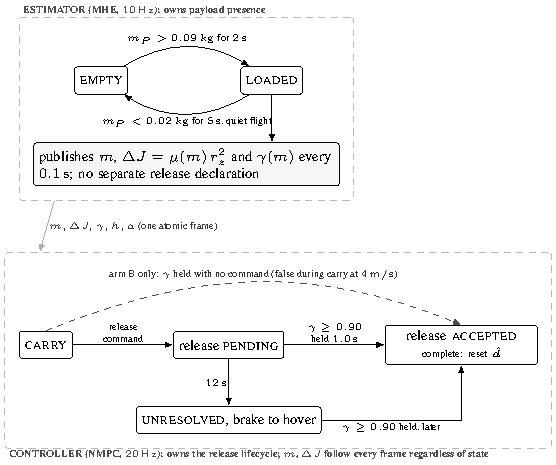
\includegraphics[width=0.92\textwidth]{Figures/fig_lifecycle_fsm_massonly.pdf}
\caption[The payload lifecycle as two state machines]{The payload lifecycle as two state machines. The estimator owns payload
presence, driven by sustained payload-mass evidence with hysteresis. The
controller owns the release lifecycle: the release command moves it from carry to
release pending and starts the \SI{12}{\second} timeout, and a release is
accepted on confirmation, $\gamma\ge0.90$ held for \SI{1.0}{\second}.
\textsc{unresolved} is a hold, not an acceptance: the vehicle brakes to hover and
keeps waiting for evidence. The dashed path exists only under the always-on
policy. In every state the mass and inertia increment follow the estimate frame
by frame; no transition sets them.}
\label{fig:fsm}
\end{figure}

Presence is a hysteretic \textsc{empty}$\leftrightarrow$\textsc{loaded} machine.
It enters \textsc{loaded} when the estimated payload mass exceeds
\SI{0.09}{\kg} for \SI{2}{\second}, with a directional thrust residual as a fast
path; it returns to \textsc{empty} when the payload mass stays below
\SI{0.02}{\kg} for \SI{5}{\second} \emph{while the vehicle is quiet}
($\lVert\bm\omega\rVert\le\SI{0.15}{\radian\per\second}$,
$\lVert\bm v_{xy}\rVert\le\SI{0.20}{\meter\per\second}$). The quiet-flight
condition is there because the mass is least reliable in manoeuvre
(Section~\ref{sec:frame:limits-lifecycle}). The thresholds differ by a factor of
four-and-a-half on purpose: the estimate is naturally low while it converges
after a grasp, and a single threshold would toggle at the start of every lift. A
separate latch records that the present flight reliably entered \textsc{loaded}
at some point.

\subsection{No-payload evidence score}\label{sec:frame:gamma}

Apart from whether a release command has been issued, every lifecycle decision
of the controller is a function of the published frame \eqref{eq:frame} alone. Let $\sigma(v;a,b)$ be the smooth indicator that is $1$
for $|v|\le a$, $0$ for $|v|\ge b$, and in between
\begin{equation}
\sigma(v;a,b) = 1 - \bigl(3\chi^2 - 2\chi^3\bigr),
\qquad \chi = \frac{|v|-a}{b-a},
\label{eq:smoothstep}
\end{equation}
which is the standard cubic smooth-step: continuous with continuous first
derivative at both ends. Let $\bar m_{P,k}$ be the estimator's filtered payload
mass and let $\gamma_k^\star$ be its instantaneous empty-payload score. The
published score is filtered once more at the output stage:
\begin{equation}
\begin{aligned}
\gamma_k^\star &= \sigma\bigl(\bar m_{P,k};\,0.015,\,0.060\bigr),\\
\gamma_k &= \gamma_{k-1}+\alpha_\gamma
              \bigl(\gamma_k^\star-\gamma_{k-1}\bigr),
\qquad
\alpha_\gamma=1-e^{-\Delta t/\SI{0.25}{\second}}.
\end{aligned}
\label{eq:gamma}
\end{equation}
Thus $\gamma$ is a deterministic evidence score, not a posterior probability or
a statistical confidence level. The score is $1$ at or below \SI{0.015}{\kg},
$0$ at or above \SI{0.060}{\kg}, and changes smoothly between them. The
instantaneous score exceeds $0.90$ below approximately \SI{0.024}{\kg}; the
additional output filter determines when the published score crosses that
threshold. The inertia increment is deliberately absent: in the mass-only model
it is a deterministic function of the same mass estimate and therefore cannot
provide independent release evidence.

\subsection{Confirmation, \textsc{unresolved}, and braking to hover}\label{sec:frame:unresolved}

The controller accepts a release through exactly one route:
\begin{equation}
\gamma \ge 0.90 \quad\text{held for}\quad \SI{1.0}{\second}
\quad\text{on healthy, fresh frames.}
\label{eq:confirm}
\end{equation}
The persistence must be contiguous in valid estimator time: a stale or failed
frame breaks the count rather than pausing it. There is no separate estimator
declaration in the evaluated configuration, and the release command does not enter
the evidence score \eqref{eq:gamma}; under the command-armed policy it only decides
when the count of \eqref{eq:confirm} may start.

If no confirmation arrives within \SI{12}{\second} of the release command, the
controller enters \textsc{unresolved}. This state is what makes confirmation on
the estimate deployable, and its semantics deserve emphasis: \textbf{a timeout is
not a release}. Nothing is accepted, the residual is not reset, and the model
continues to follow the estimate. What changes is the vehicle's exposure:
it stops flying an aggressive trajectory it may no longer have the authority to
fly, and it gives the estimator a quiet operating point in which the mass is
best observed.

The braking manoeuvre is a finite-time reference rather than an instantaneous
switch to hover, because at \SI{4}{\meter\per\second} the latter would command a
step of several metres per second. Let $\bm p_0,\bm v_0$ be the state at the
declaration and $T_b=\SI{3}{\second}$. The stopping point is chosen as the
displacement of a constant deceleration from $\bm v_0$ to rest,
\begin{equation}
\bm p_1 = \bm p_0 + \tfrac{1}{2} T_b\, \bm v_0 ,
\label{eq:brakep1}
\end{equation}
and the reference between the two is the unique quintic satisfying
$\bm p(0)=\bm p_0$, $\dot{\bm p}(0)=\bm v_0$, $\ddot{\bm p}(0)=\bm 0$,
$\bm p(T_b)=\bm p_1$, $\dot{\bm p}(T_b)=\bm 0$, $\ddot{\bm p}(T_b)=\bm 0$:
\begin{equation}
\bm p(t) = \bm p_0 + \bm v_0 t + a_3 t^3 + a_4 t^4 + a_5 t^5,
\qquad
\begin{aligned}
a_3 &= \bigl(10\,\Delta\bm p - 6 T_b \bm v_0\bigr)/T_b^3,\\
a_4 &= \bigl(-15\,\Delta\bm p + 8 T_b \bm v_0\bigr)/T_b^4,\\
a_5 &= \bigl(6\,\Delta\bm p - 3 T_b \bm v_0\bigr)/T_b^5,
\end{aligned}
\label{eq:quintic}
\end{equation}
with $\Delta\bm p=\bm p_1-\bm p_0$. Zero acceleration at both ends means the
manoeuvre begins and ends without a jump in commanded thrust, which is what
keeps the transition from itself perturbing the estimator whose evidence is being
awaited. Attitude is blended over the same interval by the smooth-step of
\eqref{eq:smoothstep}.

\subsection{Force-balance release evidence and the uncommanded-loss watchdog}\label{sec:frame:accdet}

The failure of the always-on rule (Section~\ref{sec:frame:limits-lifecycle})
lies in its evidence, not its arming: the mass estimate of the full-state
estimator, with which the rule was developed, is the one quantity that degrades in
manoeuvre (Section~\ref{sec:eval:collapse}). The reduced estimator shrinks that
bias (Section~\ref{sec:eval:reduced}) but does not turn the mass estimate into an
independent second witness. A second test of the same question needs evidence that
does not pass through the attitude, the velocity history or the rotational
model. The vertical force balance in the body frame provides it. The specific
force measured by the inertial unit along the thrust axis, $f_z$, contains no
gravity term, and with the rotor-drag term neglected it satisfies
$f_z\approx T/m$. A mass can therefore be formed from two measured signals
alone,
\begin{equation}
m_{\mathrm{acc},k}=\frac{\bar T_k}{\max\bigl(\bar f_{z,k},\,\SI{1}{\meter\per\second\squared}\bigr)},
\qquad
T_k=\textstyle\sum_i k_f\,\omega_{i,k}^2 ,
\label{eq:macc}
\end{equation}
where $\bar{(\cdot)}$ denotes a first-order low-pass with a time constant of
\SI{0.5}{\second}, applied to the thrust reconstructed from rotor speeds and to
$f_z$ alike. The lower limit on $\bar f_{z}$ guards against division in free
fall. No estimator state enters \eqref{eq:macc}; in particular, it is unaffected
by any manoeuvre-induced bias of $\hat m$, and it remains available when the
estimator's frames are unhealthy. Its weakness is the one the mass channel also
has: a relative error in $k_f$ scales $m_{\mathrm{acc}}$ one-for-one.

The evidence score has the form of \eqref{eq:gamma} with the same pair of
thresholds,
\begin{equation}
\gamma^\star_{\mathrm{acc},k}=\sigma\bigl((m_{\mathrm{acc},k}-\mB)^{+};\,0.015,\,0.060\bigr),
\label{eq:gammaacc}
\end{equation}
filtered at the output with a \SI{0.25}{\second} time constant. The score
starts at zero, because no evidence is not evidence of an empty vehicle, and it
is held rather than advanced while either signal is stale (older than
\SI{0.2}{\second}); a stale frame also breaks the persistence count of
\eqref{eq:confirm}, which is otherwise applied to $\gamma_{\mathrm{acc}}$
unchanged: $\gamma_{\mathrm{acc}}\ge0.90$ held for \SI{1.0}{\second}. Under this
rule the controller's lifecycle reads the inertial unit and the rotor speeds
directly; the statement of Section~\ref{sec:frame:gamma} that every lifecycle
decision is a function of the published frame does not hold for it, by design.

What may consume the score is decided by \emph{dual enabling}. The score is
computed throughout the flight, but a confirmation counts only when one of two
conditions holds:
\begin{enumerate}
\item a release command is pending --- the command opens confirmation at once,
as in the command-armed policy; or
\item the \emph{uncommanded-loss watchdog} is armed. It arms after the lift has
started, once fresh evidence of load, $\gamma_{\mathrm{acc}}<0.90-0.15=0.75$,
has persisted for \SI{2.0}{\second}. Once armed it is not disarmed by a rising
score --- that rise is the event it exists to detect --- and it is cleared only
at the next pickup.
\end{enumerate}
During grasp and ground support neither condition holds, so a parcel that is
attached but still resting on the ground, for which the force balance correctly
reads an empty vehicle, cannot produce an acceptance.

An acceptance with a command pending is a normal release, with the actions of
Section~\ref{sec:frame:why-eventless}. An acceptance with no command pending and
the watchdog armed is declared an \emph{uncommanded loss}. In addition to
resetting the residual specific force, the controller then zeroes the payload
geometry, ends the attach-time inertia floor and resets the inner-loop scale to
the bare-airframe value, and suppresses any later planned release, since there is
nothing left to release. It issues no gripper command, because the gripper's
state is unknown and it may be the gripper that failed.

\subsection{What a mass-only lifecycle cannot do}\label{sec:frame:limits-lifecycle}

Because \eqref{eq:gamma} is a test on the mass alone, the lifecycle inherits
every failure of that estimate. In sustained manoeuvre a low bias can carry
$\hat m_P$ below the \SI{0.024}{\kg} confirmation threshold while the payload
is attached; no rule admitting only that estimate can distinguish the collapse
from a real release. The collapse was observed with the full-state estimator; the
reduced estimator's loaded bias in manoeuvre is smaller
(Section~\ref{sec:eval:reduced}), but the argument does not depend on its
size.

The evaluated configuration holds the inertia floor until the release command,
protecting inner-loop authority but not the lifecycle. Command-arming separately
prevents carry-phase acceptance by not evaluating the release rule before a
command. The cohort supports that arming policy
(Section~\ref{sec:eval:unsignaled}), but neither mitigation corrects the mass
estimate itself. The force-balance rule of Section~\ref{sec:frame:accdet} leaves
the estimate as it is and stops asking it the release question; its own
limitation is calibration rather than manoeuvre
(Section~\ref{sec:eval:camp:thrust}).

\subsection{Threshold provenance}\label{sec:frame:thresholds}

Table~\ref{tab:thresholds} lists every lifecycle threshold and where its value
came from. None was selected against the evaluation data; all are engineering
choices whose closed-loop sensitivity has not been swept, and they are reported
as such.

\begin{table}[ht]
\centering
\caption{Lifecycle thresholds and their provenance.}
\label{tab:thresholds}
\small
\begin{tabularx}{\textwidth}{@{}p{0.30\textwidth} p{0.24\textwidth} X@{}}
\toprule
\textbf{Threshold} & \textbf{Value} & \textbf{Provenance} \\
\midrule
presence entry & $\mP>\SI{0.09}{\kg}$, \SI{2}{\second} &
below the smallest payload tested; persistence suppresses the post-grasp
convergence transient \\
presence exit & $\mP<\SI{0.02}{\kg}$, \SI{5}{\second}, quiet flight &
slow backstop; hysteresis against the entry threshold \\
no-payload evidence score & \eqref{eq:gamma}; $\gamma\ge0.90$ held \SI{1.0}{\second} & engineering choice \\
force-balance score & \eqref{eq:macc}--\eqref{eq:gammaacc}; low-pass \SI{0.5}{\second}/\SI{0.25}{\second}; fresh within \SI{0.2}{\second} & thresholds shared with \eqref{eq:gamma}; time constants an engineering choice, checked by offline replay of the earlier cohort and frozen before the campaign of Section~\ref{sec:eval:campaign} \\
loss-watchdog arming & $\gamma_{\mathrm{acc}}<0.75$ for \SI{2.0}{\second}, after lift start & engineering choice; frozen before that campaign \\
\textsc{unresolved} timeout / brake & \SI{12}{\second} / \SI{3}{\second} & engineering choice \\
\bottomrule
\end{tabularx}
\end{table}

\section{Reference Trajectory}\label{sec:frame:ref}

The evaluation trajectory is a three-dimensional Gerono lemniscate,
\begin{equation}
x_r = r\sin a, \qquad
y_r = r\sin a\cos a = \tfrac{r}{2}\sin 2a, \qquad
z_r = z_h + d_z\sin a, \qquad a = w\,t_c ,
\label{eq:fig8}
\end{equation}
with yaw commanded along the velocity vector. The crossing is not a cusp:
$\bm v=rw(\cos a,\cos2a)$ has magnitude $\sqrt2rw$ there while the planar
acceleration vanishes. The curve therefore excites coupled translation and yaw
without a velocity reversal, and the vertical term keeps the workspace compact.

After the initial hover, position amplitude and heading are introduced with the
quintic smooth step $\alpha(s)=10s^3-15s^4+6s^5$. The ramp duration satisfies
$t_{\mathrm{ramp}}\ge2.65/w$, limiting the extra velocity due to amplitude
growth, and heading is blended from the hover direction to the trajectory
tangent. This yaw blend was retained because, without it, six development
flights at \SI{4}{\meter\per\second} spent 19--25\,\% of their first
\SI{5}{\second} at the yaw-moment constraint.

\section{Online Execution Sequence}\label{sec:frame:sequence}

At every control instant the implementation performs the following sequence.

\begin{enumerate}
\item Receive and frame-convert the latest odometry.
\item Reconstruct the physical wrench from rotor speeds, \eqref{eq:phys},
averaging the \SI{250}{\hertz} samples over the estimation interval.
\item Append the measurement and the reconstructed input to the \SI{10}{\hertz}
window; re-seed by \eqref{eq:winbal} if the window must be rebuilt.
\item Solve \eqref{eq:mhe} for $\mT$ (with the full-state estimator, also the
vehicle trajectory); with the reduced estimator, apply the mass-health check
\eqref{eq:healthband}.
\item Update the presence machine and the no-payload evidence score \eqref{eq:gamma}.
\item Assemble and publish the atomic frame \eqref{eq:frame} with its health bit
and solution age.
\item In the controller: validate freshness, low-pass filter and slew-limit the
frame \eqref{eq:lpfslew}, and write $\mT$ and $\dJ$ into the model parameters
and the hover baseline \eqref{eq:hover}.
\item Evaluate confirmation \eqref{eq:confirm} and the \textsc{unresolved}
timeout; switch the reference to the braking quintic \eqref{eq:quintic} if the
timeout expires.
\item Shift the previous solution forward as a warm start and solve
\eqref{eq:nmpc}. Between solves, publish at \SI{50}{\hertz} the thrust and the
body rate interpolated along the predicted trajectory
(Section~\ref{sec:model:interface}); invert thrust to throttle by
\eqref{eq:throttleinv} and apply the body-rate scaling
\eqref{eq:omegascale}--\eqref{eq:headroomapply}.
\item Log estimates, residuals, constraint activity, solver statistics and every
lifecycle transition.
\end{enumerate}

Estimator and controller failures are handled separately and asymmetrically. An
invalid estimator solve, or an estimate outside the health band, retains the last
accepted parameter set and marks the frame unhealthy, which --- by Section~\ref{sec:frame:frame} --- freezes the
controller's model and resets its confirmation timer. An invalid controller solve
falls back to the configured safe action rather than publishing an unconstrained
command.

\section{Chapter Summary}\label{sec:frame:summary}

This chapter addressed the third and fourth research objectives: turning the
single-parameter model of Chapter~\ref{ch:model} into an estimator and a
controller that run together, and defining the release lifecycle. The three
models involved are collected in one section: the controller predicts with the
full vehicle model and the estimate-derived inertia, while the deployed estimator
keeps only the translational dynamics, with the measured attitude as a known
input, so that no rotational model error can reach the mass. The estimator is a
constrained moving-horizon problem whose only payload decision variable is the
composite mass, initialised from a window force balance, driven by the measured
thrust, and checked against a physical health band before its estimate is
released. One atomic, health-gated frame carries the mass and the inertia
increment derived from it to the controller, which updates its prediction model,
its input baseline and its inner-loop command scaling continuously from that
frame. Release acceptance is kept separate from that adaptation: it changes the
lifecycle state, resets the residual force and declares completion, and it is
gated on estimator evidence. Two properties of the design are known before any
experiment: the lifecycle rests on the mass channel alone, and the attach-time
inertia floor protects the inner loop at the price of not being released by
evidence. Chapter~\ref{ch:evaluation} measures how the complete system behaves,
including whether the always-on or the command-armed confirmation policy should
be used.

\end{spacing}
\newpage
